\documentclass[conference]{IEEEtran}
\IEEEoverridecommandlockouts
\usepackage{cite}
\usepackage{amsmath,amssymb,amsfonts}
\usepackage{algorithmic}
\usepackage{algorithm}
\usepackage{graphicx}
\usepackage{booktabs}
\usepackage{xcolor}
\usepackage{url}

\begin{document}

\title{A Behavior-Tree Framework for Channel-Aware Failure Recovery in\\
Decentralized Multi-Robot Task Allocation under Bursty Communication}

\author{\IEEEauthorblockN{Atharva Jadhav}
\IEEEauthorblockA{\textit{Collaborative Robotics and Intelligent Systems Institute} \\
\textit{Oregon State University}, Corvallis, OR, USA\\
jadhavatharva01@gmail.com}}

\maketitle

\begin{abstract}
Decentralized multi-robot task allocation (MRTA) methods such as the
Consensus-Based Bundle Algorithm (CBBA) and its event-triggered and
implicit-coordination variants stop at the \emph{allocation} decision: they
assume a robot, once it wins a task, executes it correctly. In the field,
robots fail mid-execution, and the team must \emph{detect} the failure and
re-cover the task over a lossy, bursty channel. The core difficulty is that a
silent teammate is ambiguous---it may have failed, or it may simply be
unheard during a communication outage. Standard per-node failure detectors
(fixed timeouts, the $\varphi$-accrual detector) examine each teammate's
heartbeat history in isolation, so during a correlated outage they conclude
``everyone failed'' and trigger a storm of false takeovers, each of which
places a duplicate robot on a live task. We propose a \emph{channel-aware}
failure detector that interprets silence relative to its \emph{correlation
across the team}: isolated silence (the monitor hears the rest of the team but
not~$X$) indicates a true failure, whereas correlated silence (the monitor
hears almost no one) indicates an outage and is held. Each robot estimates
channel health online and gates its failure belief by it. In simulation across
$10^{2}$--$10^{3}$ trials we show that (i)~the $\varphi$-accrual detector has a
false-alarm \emph{floor} it cannot cross under bursty loss, while our detector
reaches near-zero false takeovers; (ii)~the false-takeover gap grows
\emph{linearly with team size}, reaching $\sim$$25\times$ at $32$ robots; and
(iii)~on the detection-latency vs.\ false-alarm receiver operating curve, our
detector is Pareto-dominant in the practical operating regime. A sequential form
of the detector unifies per-node and channel-aware detection as limiting cases
and extends the advantage to a zero-miss, conflict-averse operating point that
likewise improves with team size.
\end{abstract}

\begin{IEEEkeywords}
multi-robot systems, task allocation, failure detection, fault tolerance,
communication-aware coordination.
\end{IEEEkeywords}

\section{Introduction}
Teams of robots are increasingly deployed for search-and-rescue, inspection,
and retrieval missions in which communication is intermittent, delayed, and
\emph{bursty}---links degrade together during transient outages and partial
partitions. Decentralized MRTA addresses \emph{who does what} under these
conditions, and a large body of work---CBBA, event-triggered CBBA, and
implicit/predictive coordination---produces high-quality, conflict-free
assignments even under heavy loss.

These methods, however, terminate at the allocation decision. They assume that
a robot which wins a task will carry it out. Real missions violate this
assumption: robots fail mid-task. When that happens the team must (a)~\emph{detect}
that a teammate has stopped, and (b)~\emph{re-allocate} the orphaned task. The
recovery problem is harder than allocation precisely because of the
communication channel that allocation methods treat as a nuisance: a silent
teammate is \emph{ambiguous}. It may have failed---in which case a successor
must take over---or it may be alive but temporarily unheard---in which case
taking over places two robots on one task, wasting travel and creating a
conflict.

Classical distributed-systems failure detectors resolve this ambiguity by
waiting: a fixed timeout, or the adaptive $\varphi$-accrual
detector~\cite{phiaccrual} that fits the inter-arrival distribution of the
\emph{monitored node's own} heartbeats. Both are \emph{per-node}: they look at
one teammate in isolation. Under i.i.d.\ loss this is adequate. Under
\emph{correlated} loss---a burst that silences the whole team at once---a
per-node detector sees every teammate go quiet and fires a \emph{storm} of
takeovers, each a false alarm. This failure is not a tuning artifact but a
\emph{structural} one: conditioned on a single node's heartbeat history, a dead
primary and an outage-masked live primary are statistically
indistinguishable---both produce identical, unbounded silence. The information
that separates them does not live in any one node's timeline; it lives in the
\emph{joint} silence pattern across the team. A detector that conditions on one
node at a time discards exactly the evidence the decision needs, which is why,
as we show, $\varphi$-accrual cannot be tuned below a false-alarm floor under
correlated loss.

We make the observation that silence is evidence whose meaning is set by its
\emph{correlation across the team}:
\begin{itemize}
\item \textbf{Isolated silence}---the monitor hears the rest of the team but
not~$X$---indicates that $X$ has failed; recover.
\item \textbf{Correlated silence}---the monitor hears almost no
one---indicates a local outage or partition; hold.
\end{itemize}
Each robot estimates its \emph{channel health} online (the fraction of the team
it has heard recently) and scales its failure belief by it, committing to a
takeover only when the belief exceeds a cost-calibrated threshold. The
mechanism is a drop-in front-end to any re-allocation backend.

\noindent\textbf{Contributions.}
\begin{enumerate}
\item A channel-aware, correlated-silence failure detector for discrete-task
MRTA, formulated so the channel nuisance is estimated from the whole team
rather than from the monitored node alone.
\item An empirical characterization showing the standard $\varphi$-accrual
detector has a \emph{false-alarm floor} under bursty loss, and that the
false-takeover gap to channel-aware detection \emph{grows with team size}.
\item A receiver-operating-characteristic (ROC) analysis showing the detector
is Pareto-dominant on detection latency vs.\ false alarms in the practical
regime, and that the gap propagates downstream into wasted mission energy.
\item A \emph{channel-conditioned sequential} form of the detector that unifies
the per-node timeout and the channel-aware gate as limiting cases and extends the
safe operating regime to a zero-miss, conflict-averse point whose advantage grows
with team size.
\item Identification of a per-robot \emph{heterogeneity} blind spot in
team-average channel-aware detection, and a low-cost remedy: locality-targeted,
SWIM-style indirect probing that exploits the team's predicted positions.
\end{enumerate}

\section{Related Work}
\textbf{Decentralized MRTA.} CBBA~\cite{cbba} achieves conflict-free
assignments through consensus on bundles; event-triggered
variants~\cite{cbbaetc,edcbba} reduce communication by transmitting only on
significant change. Implicit and predictive
methods~\cite{formica,implicit} avoid communication entirely by predicting
teammates' bids. Notably, these methods treat \emph{silence} as a nuisance to be
suppressed or predicted away: event-triggered schemes engineer the channel so
that absence of a message means ``no significant change,'' and predictive
schemes assume teammates are alive and reporting honestly, inferring their
\emph{intended} actions. We take the opposite stance: silence---specifically its
correlation across the team---is the primary \emph{signal}, and its meaning
(failure vs.\ outage) is exactly what must be decoded. All of the above address
allocation and stop at the allocation decision; none treat a teammate that fails
mid-task, and none use negative information as a first-class trigger.

\textbf{Failure detection.} The $\varphi$-accrual
detector~\cite{phiaccrual} is the standard adaptive detector; it estimates the
arrival distribution of a single monitored process. Gossip-based membership
protocols such as SWIM~\cite{swim} reduce false positives with \emph{indirect
probing}---confirming a suspected node through other members before declaring it
failed---a mechanism we adopt (in a locality-targeted form) to handle per-robot
link heterogeneity in Section~\ref{sec:relay}. Network- and context-aware
detectors exist in distributed systems, but discrete-task MRTA recovery under
correlated loss, with an explicit cost for duplicate-robot conflicts, is not
addressed. The closest MRTA work detects danger through observation of the
environment rather than through the correlation structure of silence. Our
detector is the \emph{channel-coupled} analogue of $\varphi$-accrual: where
$\varphi$-accrual estimates the monitored node's own statistics, we estimate the
\emph{shared channel} from the team.

\section{Problem Formulation}
A team of $N$ robots $\mathcal{R}=\{1,\dots,N\}$ must service a set of
$K$ tasks $\mathcal{T}=\{1,\dots,K\}$, $K<N$. Each robot $r$ has a cost
$c_{r,k}\ge 0$ for task $k$ (here, travel time plus a capability penalty).
An initial assignment $\pi:\mathcal{T}\!\to\!\mathcal{R}$ designates a
\emph{primary} $\pi(k)$ for each task; the remaining idle robots are ranked as
\emph{successors}. A primary may \emph{fail} at an unknown time $t^{f}_{k}$
during execution, after which it emits no further signals.

\textbf{Communication.} Time is slotted at the heartbeat period $h$. Every
alive robot $j$ broadcasts a heartbeat each slot. A message from $j$ is
received by $s$ in slot $t$ with probability $1-d(t)$, where $d(t)$ is governed
by a two-state Gilbert--Elliott channel that alternates between a \emph{good}
state (drop probability $d_{g}$) and a \emph{bad} state (drop probability
$d_{b}\!\gg\!d_{g}$), modelling correlated outages. Setting the transition
probabilities to keep the channel in one state recovers i.i.d.\ loss.

\textbf{Objective.} Each task's successor must decide, from the heartbeats it
receives, whether its primary has failed and it should take over. A takeover of
a \emph{failed} primary is a \emph{correct recovery} with detection latency
$\ell = t^{\text{takeover}} - t^{f}_{k}$. A takeover of an \emph{alive} primary
is a \emph{false takeover}, costing $c_{\text{conf}}$ (a duplicate robot on a
live task). A failed primary never taken over is a \emph{coverage hole},
costing $c_{\text{miss}}$. We seek a decision rule minimizing the expected
mission cost
\begin{equation}
J = c_{\text{conf}}\, \mathbb{E}[n_{\text{false}}]
  + c_{\text{miss}}\, \mathbb{E}[n_{\text{miss}}]
  + \lambda\, \mathbb{E}[\ell],
\label{eq:cost}
\end{equation}
where $\lambda$ trades detection speed against the two error types.

\section{Channel-Aware Failure Recovery}
\subsection{Channel health and failure belief}
Let $s$ monitor primary $p=\pi(k)$. Define the \emph{silence}
$\sigma(t)=t-\tau_{\text{last}}(s,p,t)$, where $\tau_{\text{last}}$ is the
emission time of the most recent heartbeat from $p$ received by $s$. Define the
\emph{channel health} as the fraction of the \emph{other} teammates $s$ has
heard within a window $W$:
\begin{equation}
\eta(s,p,t) = \frac{1}{N-2}\!\!\sum_{j\neq s,p}\!\!
\mathbf{1}\!\left[\,\tau_{\text{last}}(s,j,t) \ge t-W\,\right].
\label{eq:health}
\end{equation}
A normalized silence severity is
$\rho(t)=\mathrm{clip}\!\left((\sigma(t)-2h)/4h,\,0,\,1\right)$, and the
\emph{failure belief} couples the two signals multiplicatively:
\begin{equation}
\beta(s,p,t) = \rho(t)\cdot \eta(s,p,t).
\label{eq:belief}
\end{equation}
The coupling encodes the principle directly: long silence ($\rho\!\to\!1$)
indicates failure \emph{only when} the rest of the team is heard
($\eta\!\to\!1$). During a correlated outage $\eta$ collapses and the belief is
suppressed regardless of how long $p$ has been silent. The successor takes over
the instant
\begin{equation}
\beta(s,p,t) \ge \tau, \qquad
\tau = \frac{c_{\text{conf}}}{c_{\text{miss}}+c_{\text{conf}}},
\label{eq:thresh}
\end{equation}
where $\tau$ is the cost-optimal threshold derived from
\eqref{eq:cost}: balanced costs give $\tau=0.5$; costly misses lower $\tau$ so
the successor acts eagerly; costly conflicts raise it so it holds.

\subsection{Why channel health is the right conditioning variable}
The multiplicative coupling in \eqref{eq:belief} is not arbitrary; it
approximates the posterior probability that $p$ has failed given the observed
silence. Write $F$ for the event ``$p$ failed.'' Long silence from $p$ can arise
two ways: $p$ is dead, or the link to $p$ is in a bad state. Under the
correlated channel, the link state of $p$ is not independent of the links to the
rest of the team---a burst that drops $p$ tends to drop everyone. The fraction
of \emph{other} teammates heard, $\eta$, is therefore a sufficient statistic for
the latent channel state as seen by $s$: when $\eta\!\to\!1$ the channel is
almost surely good, so silence from $p$ is overwhelmingly explained by failure
($\Pr[F\mid\sigma,\eta]\!\to\!1$); when $\eta\!\to\!0$ the channel is almost
surely bad, so silence is explained away ($\Pr[F\mid\sigma,\eta]\!\to\!0$). The
product $\rho\cdot\eta$ is the simplest estimator with these two limits and
monotone in between; we deliberately avoid a tuned parametric posterior so the
contribution is the \emph{conditioning principle}, not a fitted curve. Crucially,
$\eta$ is observable by every successor with no extra communication---it is a
by-product of the heartbeats already received---so the team-level evidence is
available locally and online.

\begin{algorithm}[t]
\caption{Channel-aware takeover decision (run by successor $s$ for task $k$)}
\label{alg:detect}
\begin{algorithmic}[1]
\REQUIRE heartbeat receptions; primary $p$; window $W$; threshold $\tau$
\STATE \textbf{at each slot } $t$:
\STATE $\sigma \gets t - \tau_{\text{last}}(s,p,t)$
       \hfill$\triangleright$ silence from $p$
\STATE $\rho \gets \mathrm{clip}\big((\sigma-2h)/4h,\,0,\,1\big)$
\STATE $\eta \gets$ fraction of other teammates heard in $[t-W,t]$
       \hfill$\triangleright$ Eq.~\eqref{eq:health}
\STATE $\beta \gets \rho\cdot\eta$ \hfill$\triangleright$ failure belief
\IF{$\beta \ge \tau$}
    \STATE \textbf{trigger} re-allocation of task $k$; \textbf{stop}
\ENDIF
\end{algorithmic}
\end{algorithm}

\subsection{Re-allocation backend}
Detection is a front-end; once a takeover is triggered the orphaned task is
re-allocated by the \emph{incremental} routine of Algorithm~\ref{alg:backend}.
Only \emph{truly-available} robots bid---those not already committed to another
recovery and either idle from the outset or having finished their own
(non-failed) task by the trigger time---and the lowest-cost available bidder
commits after a bounded mini-consensus among the bidders. We stress that this
backend is \emph{not} a contribution: it is standard incremental auctioning,
and we present it only for reproducibility and to make explicit that it is
\textbf{held fixed across every detector we compare}. Because the same backend
processes the output of \texttt{fixed\_timeout}, $\varphi$-accrual,
\texttt{channel\_aware}, and our detector identically, any difference in the
metrics of Section~\ref{sec:exp} is attributable solely to the decision rule of
Algorithm~\ref{alg:detect}, not to the re-allocation mechanics.

\begin{algorithm}[t]
\caption{Incremental re-allocation backend (held fixed across all detectors)}
\label{alg:backend}
\begin{algorithmic}[1]
\REQUIRE orphaned task $k$ at trigger time $t$; per-robot costs $c_{r,k}$;
         set of committed robots $\mathcal{C}$
\STATE $\mathcal{A} \gets \{\,r \notin \mathcal{C} : r \text{ idle, or }
       r\text{'s own task finished and not failed by }t\,\}$
       \hfill$\triangleright$ truly available
\IF{$\mathcal{A} = \emptyset$}
    \STATE \textbf{return} uncovered \hfill$\triangleright$ no spare capacity
\ENDIF
\STATE run bounded mini-consensus over $\mathcal{A}$ on $\{c_{r,k}\}$
       (max $R$ rounds, lossy channel)
\STATE $r^{\star} \gets \arg\min_{r\in\mathcal{A}} c_{r,k}$
\IF{consensus did not converge within $R$}
    \STATE flag conflict \hfill$\triangleright$ a duplicate bidder may also act
\ENDIF
\STATE commit $r^{\star}$: $\mathcal{C}\gets\mathcal{C}\cup\{r^{\star}\}$;
       complete at $t + \text{(consensus delay)} + \text{travel} + \text{exec}$
\end{algorithmic}
\end{algorithm}

\section{Experiments}
\label{sec:exp}
We simulate $N$ robots and $K$ tasks under the Gilbert--Elliott channel. All
detectors share one stochastic channel realization per trial and the same
incremental backend; only the decision rule varies. We compare against
\texttt{fixed\_timeout}, the $\varphi$-accrual detector
(\texttt{adaptive\_pernode}), and a simpler channel-aware timeout
(\texttt{channel\_aware}) that inflates a timeout by $(1-\eta)$ rather than
forming a belief. Unless noted: $d_{g}=0.2$, burst channel, $h=0.75$\,s,
$400$--$600$ trials.

\subsection{End-to-end comparison: success, completion time, wasted effort}
\label{sec:e2e}
We first compare whole-mission outcomes ($K{=}6$ tasks, $N{=}12$ robots,
$p_{\text{fail}}{=}0.4$, burst; Table~\ref{tab:e2e}, Fig.~\ref{fig:comparison}).
Three points stand out. (i)~\textbf{Recovery is necessary}: an allocation-only
baseline that never recovers (the regime of CBBA and its event-triggered and
implicit variants) completes only $59\%$ of tasks, and this collapses further as
the failure rate rises (Fig.~\ref{fig:comparison}d), whereas every recovery
method reaches $100\%$. (ii)~\textbf{Recovery is affordable}: all recovery
methods finish in comparable time ($15.5$--$17.8$\,s); the per-node detectors are
in fact marginally faster, because they act hastily---which is precisely the
cost in (iii). (iii)~\textbf{The separator is wasted effort}: the per-node
detectors pay for their haste with $0.98$--$1.27$ false takeovers per trial and
$7.7$--$9.6$ units of wasted travel, while the channel-aware methods (the simple
timeout and our belief, which behave almost identically here) incur $\sim$$0.08$
false takeovers and $<\!0.7$ wasted travel---a $\sim$$16\times$ reduction in
duplicate-robot conflicts at the same success rate and comparable completion
time. Mission success and completion time thus establish that recovery is needed
and cheap; the remaining sections isolate \emph{how cleanly} each detector
achieves it, which is where channel-awareness and team size matter. We stress
that the channel-aware timeout is not a competing method but the \emph{simplest
member of our channel-aware family}: it uses the same team-estimated signal
$\eta$. The meaningful contrast is therefore between this family and the per-node
baselines (here, $\sim$$16\times$), and---once the channel is \emph{graded}
rather than bimodal---between the full belief and the simple timeout
(Section~\ref{sec:partition}).

\begin{table}[t]
\caption{End-to-end comparison (burst, $K{=}6$, $N{=}12$, $p_{\text{fail}}{=}0.4$,
$500$ trials). All recovery methods succeed; they differ in wasted effort.}
\label{tab:e2e}
\centering
\small
\begin{tabular}{lccccc}
\toprule
method & succ.\ & recov.\ & time & false & energy\\
       & (\%)   & (\%)    & (s)  & tk.\  & \\
\midrule
no recovery (alloc-only) & 59.1 & 4.0 & 6.6 & 0.00 & 0.00\\
fixed timeout            & 100  & 100 & 15.7 & 0.98 & 7.71\\
$\varphi$-accrual        & 100  & 100 & 15.5 & 1.27 & 9.55\\
channel-aware timeout    & 100  & 100 & 17.8 & 0.07 & 0.54\\
\textbf{ours (belief)}   & 100  & 100 & 17.4 & \textbf{0.08} & \textbf{0.70}\\
\bottomrule
\end{tabular}
\end{table}

\begin{figure}[t]
\centering
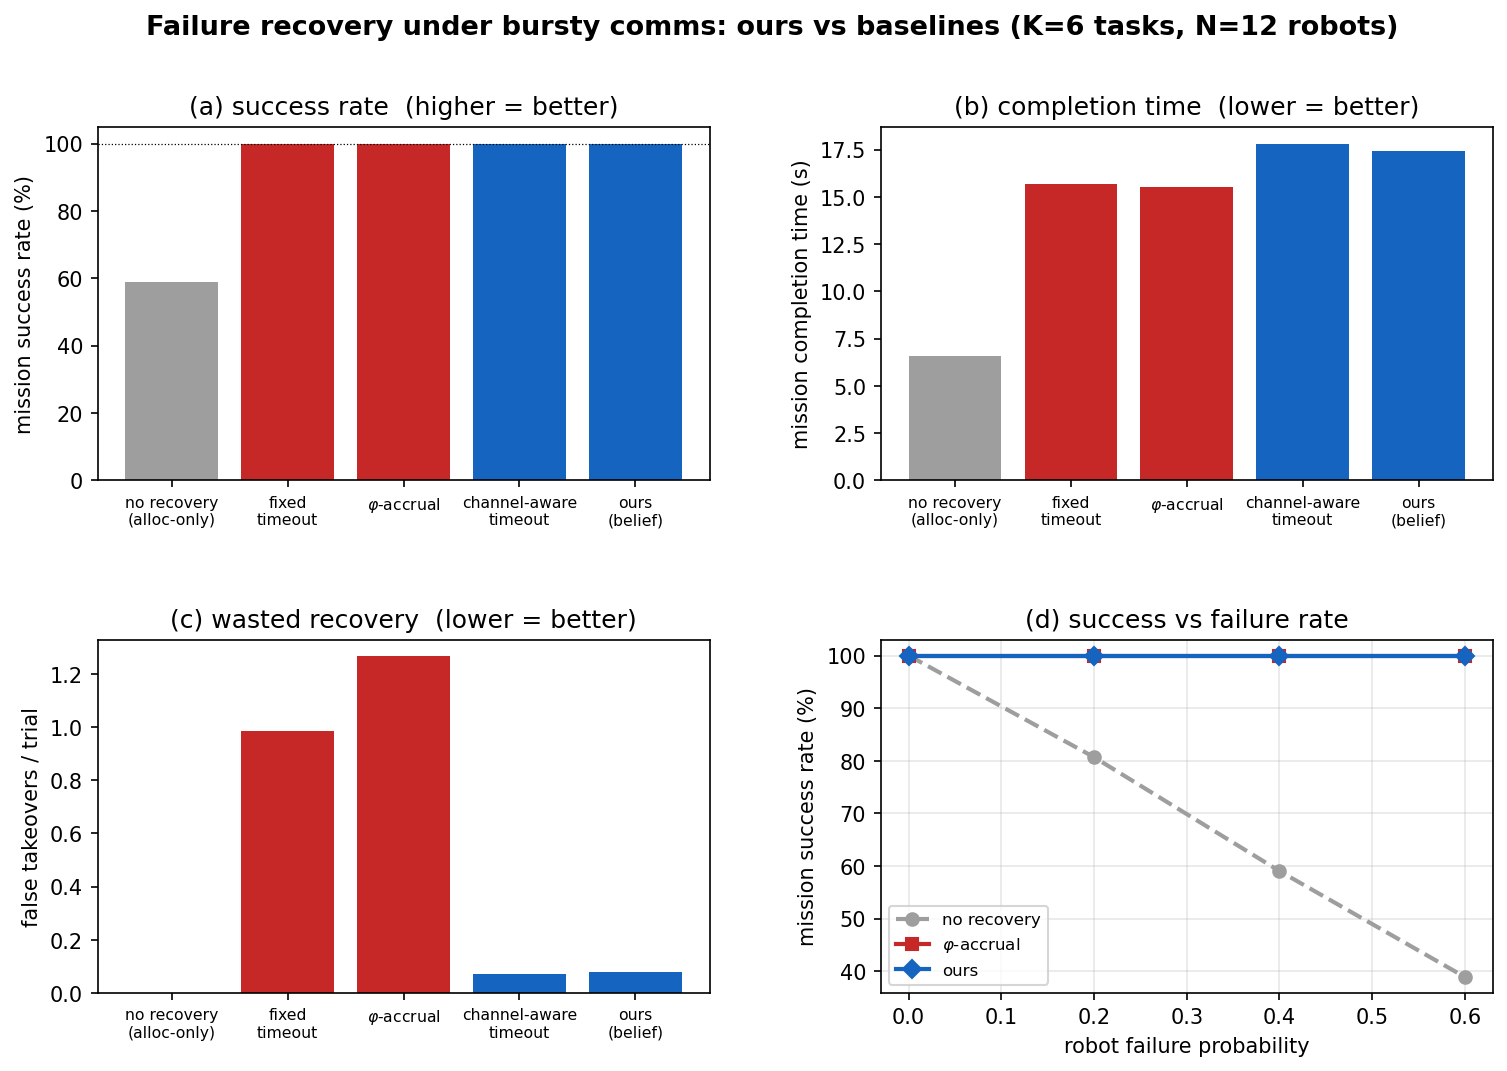
\includegraphics[width=\columnwidth]{fig_comparison.png}
\caption{End-to-end comparison (burst). (a)~mission success rate---recovery
lifts $59\%\!\to\!100\%$; (b)~completion time---comparable across recovery
methods; (c)~wasted recovery---per-node detectors incur $\sim$$16\times$ more
false takeovers than the channel-aware methods; (d)~success vs.\ failure
rate---allocation-only collapses, recovery stays at $100\%$.}
\label{fig:comparison}
\end{figure}

\subsection{The per-node false-takeover storm scales with team size}
Figure~\ref{fig:scale} sweeps team size. The per-node detectors' false
takeovers grow roughly linearly---$\varphi$-accrual rises from $0.70$ to
$2.49$ per trial as the team grows from $6$ to $32$ robots---because each
additional monitored primary contributes another independent false alarm during
a burst. Channel-aware detection stays flat ($\sim$$0.08$--$0.10$). The gap
widens from $\sim$$9\times$ to $\sim$$25\times$.

\begin{figure}[t]
\centering
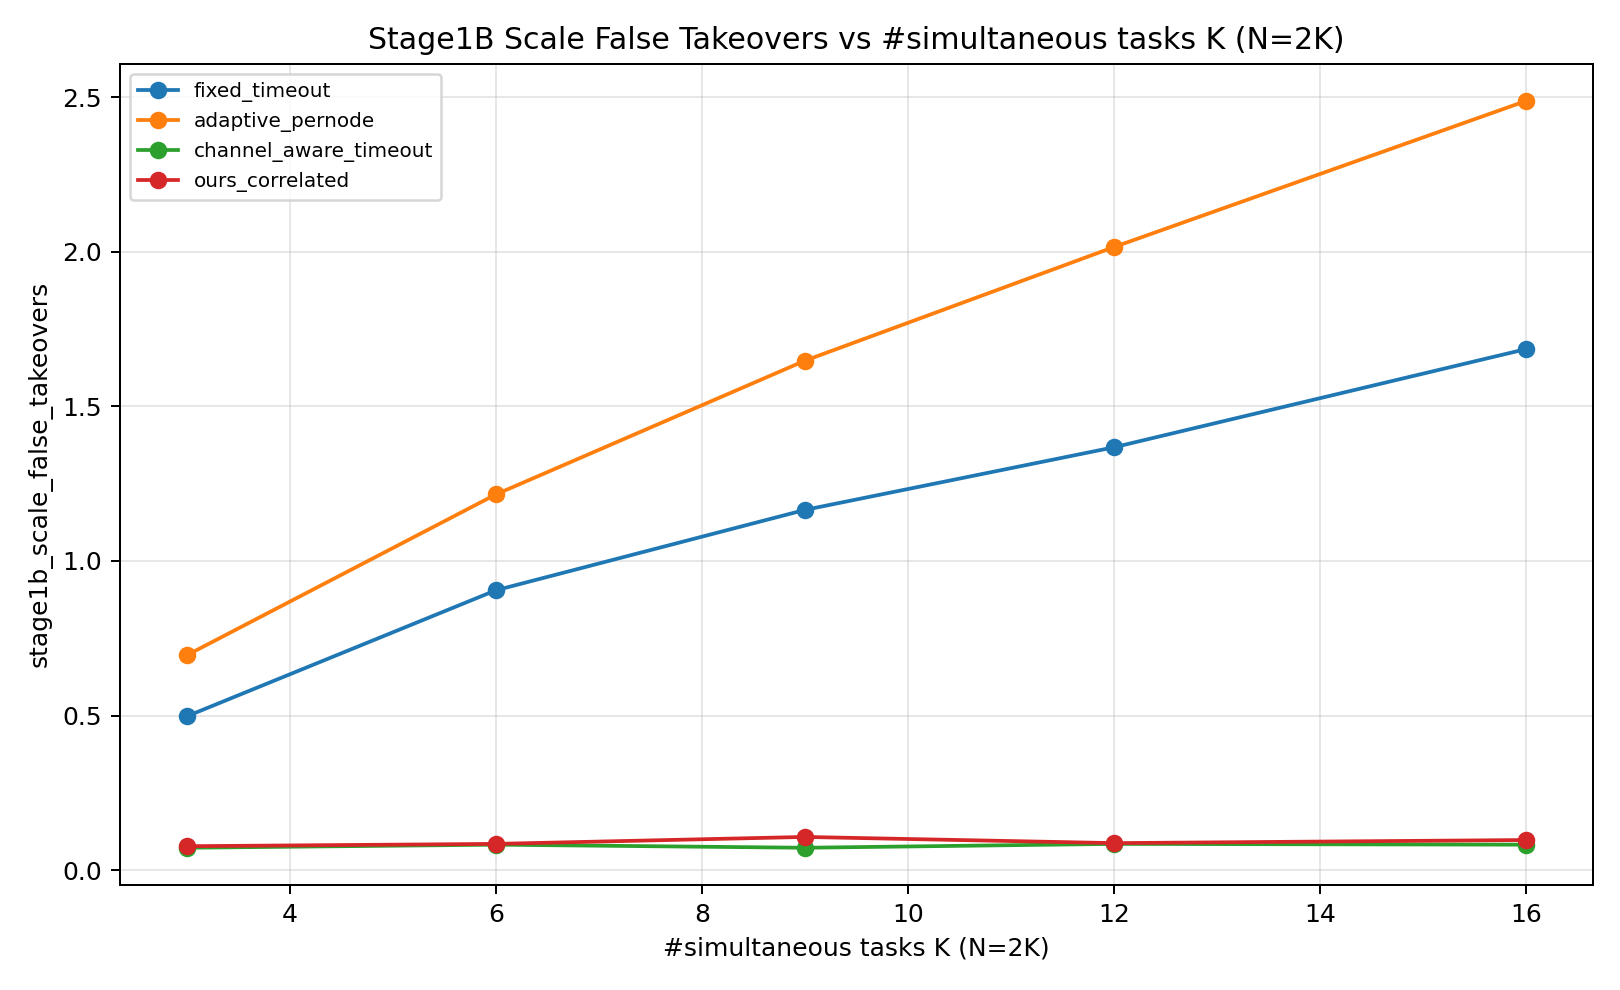
\includegraphics[width=\columnwidth]{fig_scale.png}
\caption{False takeovers per trial vs.\ team size (burst channel). Per-node
detectors (fixed timeout, $\varphi$-accrual) storm linearly; channel-aware
detection stays flat. The advantage grows with the team.}
\label{fig:scale}
\end{figure}

\subsection{ROC: a structural speed/accuracy advantage}
A per-node detector has a single knob---how long to wait---and cannot
distinguish a dead node from a bad channel, so it is confined to a poor
speed/accuracy trade-off. Sweeping each detector's sensitivity across its full
range traces the ROC of Fig.~\ref{fig:roc}. Two findings stand out. First, the
$\varphi$-accrual detector has a \emph{false-alarm floor}: under burst it cannot
fall below $0.46$ false takeovers per trial no matter how conservatively it is
tuned, while its latency balloons. The floor is stubborn. Extending the
sensitivity sweep far past the range plotted---from $k=14$ to $k=120$ standard
deviations---leaves the false-takeover rate unchanged to the resolution of the
sweep, while mean detection latency grows from $5.3$\,s to $14.2$\,s and the
detector then begins missing real failures outright (recovery falls from
$100\%$ to $55\%$). No tuning escapes it.

It is worth being precise about what does and does not cause this, because the
obvious generalisation is wrong. The floor is \emph{not} a property of per-node
detection as such: a fixed timeout is equally per-node, and it does reach zero
false takeovers---at a multiplier of $16$, with full recovery and a detection
latency of $11.4$\,s, roughly three times ours at a comparable false-alarm rate. The floor
belongs specifically to the \emph{adaptive} detector, and its adaptation is the
liability. $\varphi$-accrual sets each teammate's threshold from the variance of
that teammate's \emph{observed} inter-arrival gaps---and a burst contributes no
samples, so the statistic it adapts to is built from the traffic that got
through. Teammates whose delivered heartbeats look most regular are assigned the
tightest thresholds, and are then precisely the teammates a burst silences.
Scaling $k$ inflates every threshold but does not repair the ranking, which is
why latency degrades while the false alarms persist. Channel health supplies the
axis the per-node statistic is missing, which is why our detector reaches the
low-false-alarm region without paying the fixed timeout's latency. Second, in the practical low-false-alarm
regime our detector is Pareto-dominant: at a matched false-alarm rate it detects
real failures $\sim$$15$--$20\%$ faster than the channel-aware timeout and
$\sim$$30$--$45\%$ faster than the fixed timeout (Table~\ref{tab:roc}), because
the belief fires quickly the instant the channel is good while a timeout waits a
fixed multiple regardless.

\begin{figure}[t]
\centering
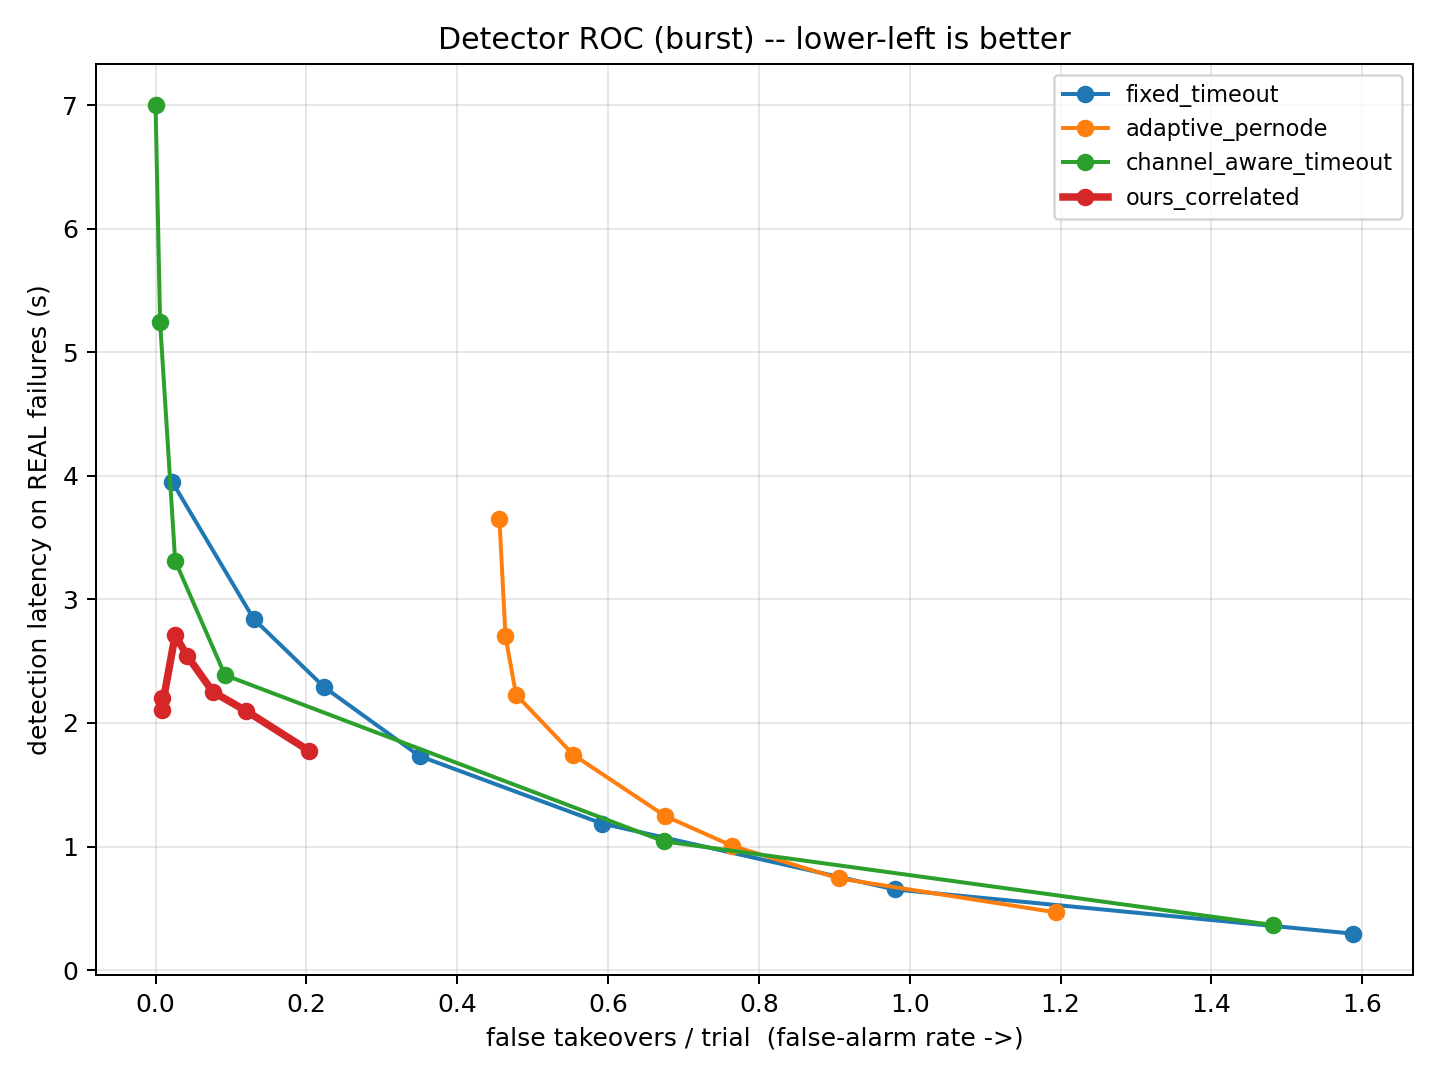
\includegraphics[width=\columnwidth]{fig_roc.png}
\caption{Detector ROC (burst). Lower-left is better. Our detector lies below
all baselines in the practical regime; $\varphi$-accrual cannot reach the
low-false-alarm region at any sensitivity, including settings far beyond those
plotted.}
\label{fig:roc}
\end{figure}

\begin{table}[t]
\caption{Detection latency (s) at matched false-alarm rate (burst).
$\varphi$-accrual cannot reach these rates.}
\label{tab:roc}
\centering
\begin{tabular}{ccccc}
\toprule
false alarms/trial & fixed & $\varphi$-accrual & chan.-aware & \textbf{ours}\\
\midrule
0.20 & 2.43 & --- & 2.14 & \textbf{1.79}\\
0.10 & 3.15 & --- & 2.37 & \textbf{2.17}\\
0.05 & 3.66 & --- & 2.98 & \textbf{2.47}\\
0.03 & 3.87 & --- & 3.26 & \textbf{2.67}\\
\bottomrule
\end{tabular}
\end{table}

\subsection{The detection gap propagates to wasted energy}
The false-takeover storm is not a bookkeeping quantity: every false takeover
sends a second robot driving to a task that did not need it, and that travel is
pure wasted energy. Figure~\ref{fig:energy} sweeps team size and reports the
mean wasted travel---the successor distance spent on false
takeovers---per trial. Because wasted energy is, to first order, the
false-takeover count times the average travel-to-task, it inherits and amplifies
the storm: the per-node detectors waste $4$--$15$ travel units per trial and
\emph{grow} with the team ($\varphi$-accrual rises from $5.6$ at $K{=}3$ to
$15.2$ at $K{=}16$), while both channel-aware detectors stay flat below~$1$
($\sim$$20\times$ less at $K{=}16$). The structural advantage of conditioning on
the team thus shows up directly in a physical mission cost.

We deliberately do \emph{not} claim a raw makespan or detection-latency
advantage at a fixed sensitivity: a per-node detector that fires eagerly
\emph{appears} faster precisely because it does not wait to disambiguate, paying
for that speed in the false takeovers of Fig.~\ref{fig:energy}. The fair
speed comparison is at a matched false-alarm rate, which is exactly the ROC of
Fig.~\ref{fig:roc} and Table~\ref{tab:roc}; there our detector is faster.

\begin{figure}[t]
\centering
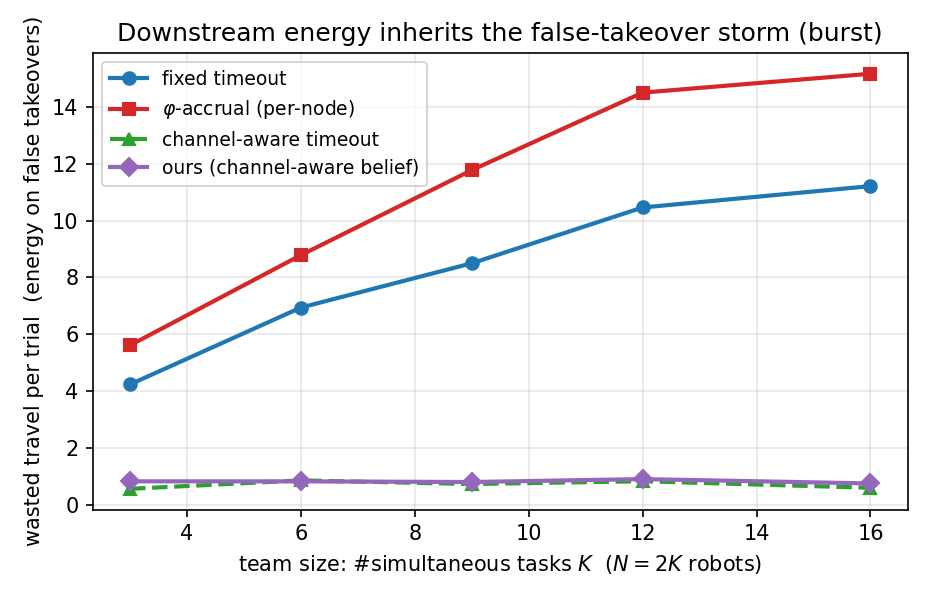
\includegraphics[width=\columnwidth]{fig_energy.png}
\caption{Wasted travel (energy spent on false takeovers) per trial vs.\ team
size (burst). The per-node detectors' wasted energy grows with the team;
channel-aware detection stays near zero. The downstream cost inherits the
detection gap.}
\label{fig:energy}
\end{figure}

\subsection{Partial partitions}
\label{sec:partition}
The full-burst comparison of Section~\ref{sec:e2e} is the regime \emph{least}
favourable to the belief: there channel health is bimodal ($0/1$), so the
continuous belief and the simple channel-aware timeout make the same decision.
The belief's value appears precisely where channel health is \emph{graded}---a
transient group split that leaves a successor hearing only part of the team
(channel health near $0.5$), so an alive cross-partition primary looks silent.
Figure~\ref{fig:partition} sweeps the severity of such a split. The continuous
belief separates failed from partitioned-but-alive primaries markedly better than
a hard timeout: at a mild split it incurs $0.018$ false takeovers on alive
robots, against $0.040$ for the simple channel-aware timeout ($2.2\times$ fewer)
and $0.085$ for $\varphi$-accrual ($4.6\times$ fewer); the ordering
$\varphi\text{-accrual} > \text{fixed} > \text{simple} > \text{belief}$ holds
across severities. This is the regime the sequential test of
Section~\ref{sec:seq} is designed to exploit further.

\begin{figure}[t]
\centering
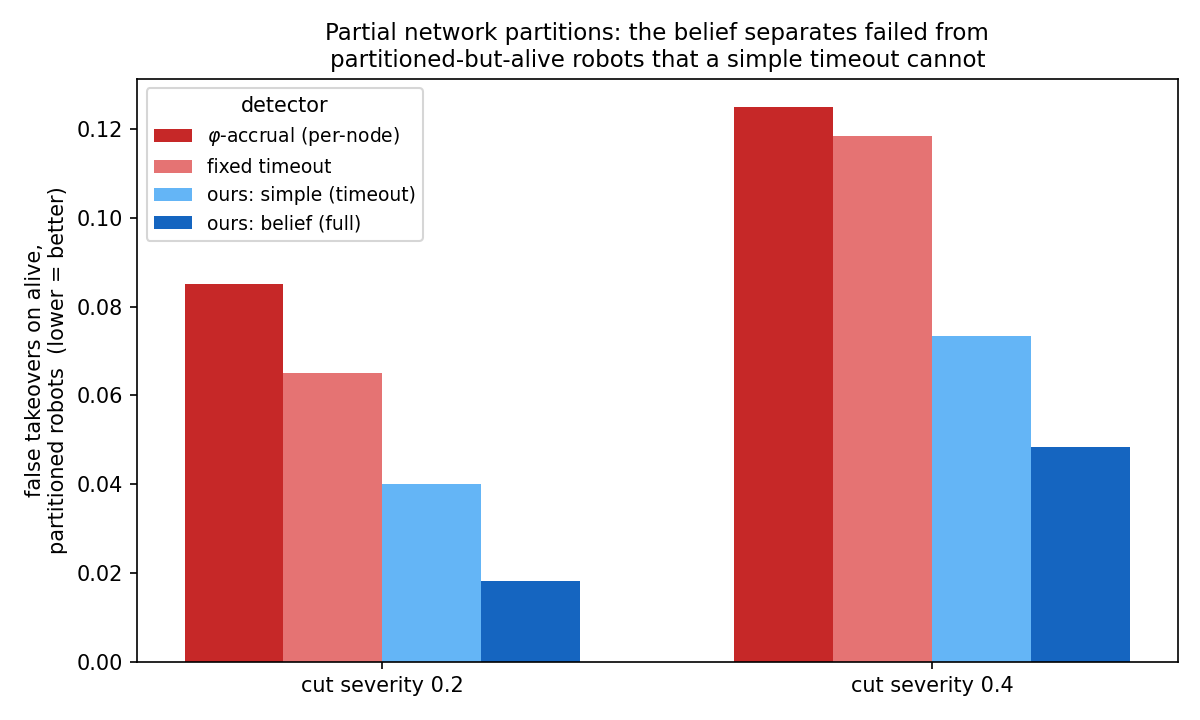
\includegraphics[width=\columnwidth]{fig_partition_gap.png}
\caption{Partial network partitions (graded channel health). False takeovers on
alive-but-partitioned robots: the continuous \emph{belief} (dark) separates
failed from temporarily-cut-off robots that a simple timeout cannot, beating the
simple channel-aware timeout $\sim$$2\times$ and the per-node detectors
$\sim$$3$--$5\times$.}
\label{fig:partition}
\end{figure}

\subsection{A sequential test extends the safe operating regime}
\label{sec:seq}
The instantaneous belief of \eqref{eq:belief} is bounded by $\eta$, so in the
\emph{conflict-averse} regime---where a duplicate-robot conflict is so costly
that one demands an ultra-low false-alarm rate---it must eventually trade
coverage for safety. We therefore promote the detector to a
\emph{channel-conditioned sequential test}: the successor accumulates per-slot
evidence
\begin{equation}
L(t)=\sum_{\tau\le t}\; -\log\!\big(1-\eta(\tau)\big),
\label{eq:seq}
\end{equation}
weighting each missed heartbeat by the instantaneous channel health, and takes
over when $L(t)\ge\Lambda$. Because an outage drives $\eta\!\to\!0$, its slots
contribute no evidence (the burst is explained away), whereas good-channel slots
contribute strongly; and because $L$ is \emph{unbounded}, any safety threshold is
reachable by accumulating evidence over time. The formulation is also unifying:
the per-node timeout and the channel-aware gate of Section~\ref{sec:exp} are its
constant-$\eta$ and single-slot limits.

This removes the coverage cost in the safe regime. Figure~\ref{fig:seq} contrasts
the two: as the operating point is pushed toward zero false alarms, the bounded
belief begins to miss real failures, while the sequential test holds missed
failures at essentially zero across the whole frontier. The effect is decisive at
scale: at $32$ robots and a matched false-alarm rate of $0.02$, the bounded belief
misses a significant fraction of failures ($0.15$, $95\%$ CI $[0.06,0.87]$ over
$B{=}4000$ paired bootstrap resamples), whereas the sequential test misses
essentially none ($0.00$, $[0.00,0.02]$) at the \emph{same} false-alarm rate. It
is thus the only detector that reaches the conflict-averse regime without losing
coverage (Table~\ref{tab:seq}). Among the full-coverage detectors, its detection
latency matches or modestly beats the channel-aware timeout ($3.92$ vs.\ $4.33$\,s
at FA$=0.05$; faster in $97\%$ of resamples, though the latency gap alone is not
significant at $95\%$), with a tighter latency distribution; this separation
emerges only as the team grows, the two being comparable at small teams.

\begin{figure}[t]
\centering
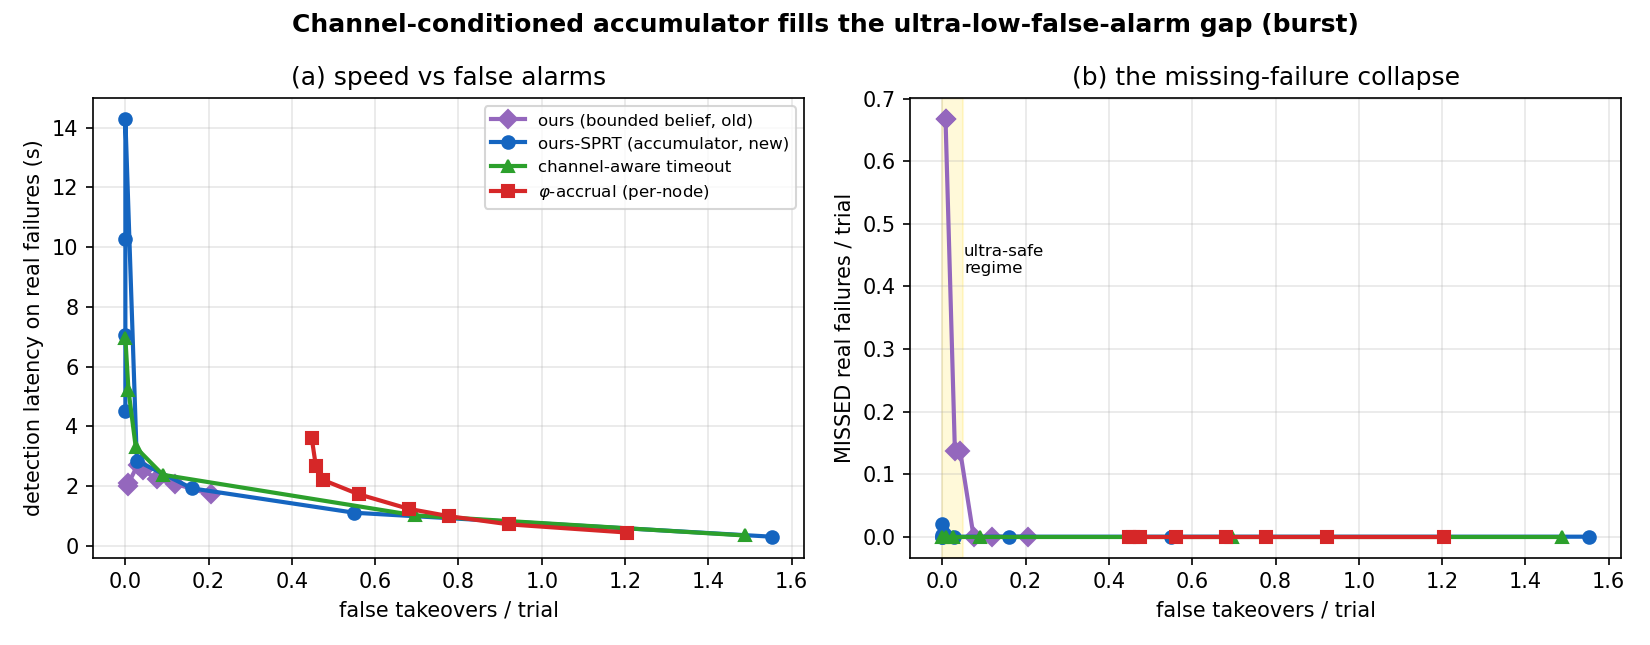
\includegraphics[width=\columnwidth]{fig_sprt.png}
\caption{Sequential test vs.\ the bounded belief (burst). (a)~speed--false-alarm
frontier; (b)~as the operating point approaches zero false alarms the bounded
belief misses failures, while the sequential test stays at $\sim$$0$ missed
across the frontier.}
\label{fig:seq}
\end{figure}

\begin{table}[t]
\caption{Matched-false-alarm comparison at $32$ robots (burst) with $95\%$
paired-bootstrap CIs ($B{=}4000$, $N{=}500$ trials). In the conflict-averse
regime the bounded belief loses coverage (missing $0.15$ of failures at
FA${=}0.02$), whereas the sequential test maintains \emph{full coverage} at
latency comparable to the channel-aware timeout.}
\label{tab:seq}
\centering
\begin{tabular}{llcc}
\toprule
FA & detector & latency (s) [95\% CI] & missed/trial [95\% CI]\\
\midrule
$0.05$ & channel-aware  & $4.33\ [3.9,5.7]$ & $0.00\ [0.00,0.00]$\\
       & bounded belief & $3.76\ [3.5,4.0]$ & $0.01\ [0.00,0.09]$\\
       & \textbf{sequential} & $3.92\ [3.8,4.1]$ & $\mathbf{0.00\ [0.00,0.00]}$\\
\midrule
$0.02$ & channel-aware  & $4.96\ [4.7,7.2]$ & $0.00\ [0.00,0.00]$\\
       & bounded belief & $4.19\ [4.0,4.4]$ & $0.15\ [0.06,0.87]$\\
       & \textbf{sequential} & $4.07\ [3.9,10.5]$ & $\mathbf{0.00\ [0.00,0.02]}$\\
\bottomrule
\end{tabular}
\end{table}

\subsection{Per-robot link heterogeneity, and a locality-targeted remedy}
\label{sec:relay}
Channel health $\eta$ is a \emph{team-average}, which exposes a blind spot: it
cannot see a \emph{single} robot whose own link is uniquely bad. Consider an
alive primary $X$ that is occluded from its monitor~$S$ (a poor $X$--$S$ link)
while the rest of the team is clear to~$S$. Then $\eta$ stays high, $S$ concludes
``the channel is fine, so the silent $X$ must have failed,'' and recovers a live
robot. This is not specific to our rule: with one robot's drop rate raised while
the team stays clear, \emph{every} detector studied here false-recovers the alive
robot once that link exceeds $\sim$$0.5$ (rate $\to$$1.0$), and channel-awareness
confers no protection, because the damaging silence is not correlated across the
team.

The remedy is to complement the local channel-health signal with \emph{second-hand
liveness}: rather than ask ``can \emph{I} hear $X$?'', ask ``can \emph{anyone}
hear $X$?''---SWIM-style indirect probing~\cite{swim}, in which suspected nodes
are confirmed through other members before being declared failed. Our setting
admits a cheap, \emph{locality-targeted} instance: each robot already broadcasts
its assignment, so the team maintains predicted positions, and because physical
proximity correlates with link quality, $S$ queries only the $k$ robots predicted
\emph{nearest} the silent~$X$ instead of flooding the team. Figure~\ref{fig:relay}
reports both axes. Targeted probing ($k{=}2$) suppresses $\sim$$97\%$ of the
heterogeneity-induced false takeovers ($1.00\!\to\!0.03$), matching a full flood,
at roughly one-sixth of its message cost ($31$ vs.\ $175$ messages/trial); and it
degrades \emph{gracefully} as the position model goes stale---still $0.28$ (vs.\
the no-remedy $1.0$) even when $80\%$ of position updates are lost. The
contribution here is not the indirect-probe mechanism, which is SWIM's, but the
identification of the team-average detector's per-robot blind spot and the
demonstration that a locality-targeted probe closes it at low cost
(Algorithm~\ref{alg:relay}).

\begin{algorithm}[t]
\caption{Locality-targeted recovery (monitor $s$, suspected primary $p$)}
\label{alg:relay}
\begin{algorithmic}[1]
\REQUIRE suspicion fired for $p$ (Alg.~\ref{alg:detect}); predicted positions
         $\hat{x}_j$; probe fan-out $k$
\STATE $Q \gets$ the $k$ robots minimizing $\lVert \hat{x}_j-\hat{x}_p\rVert$
       \hfill$\triangleright$ predicted nearest to $p$, not to $s$
\STATE query each $j\in Q$: ``heard $p$ within window $W$?''
\IF{any $j\in Q$ replies yes}
    \STATE $p$ is alive (a local bad link to $s$);
           \textbf{cancel} and resume monitoring
\ELSE
    \STATE $p$ \textbf{confirmed failed}: trigger re-allocation of its task
           (Alg.~\ref{alg:backend})
\ENDIF
\end{algorithmic}
\end{algorithm}

\begin{figure}[t]
\centering
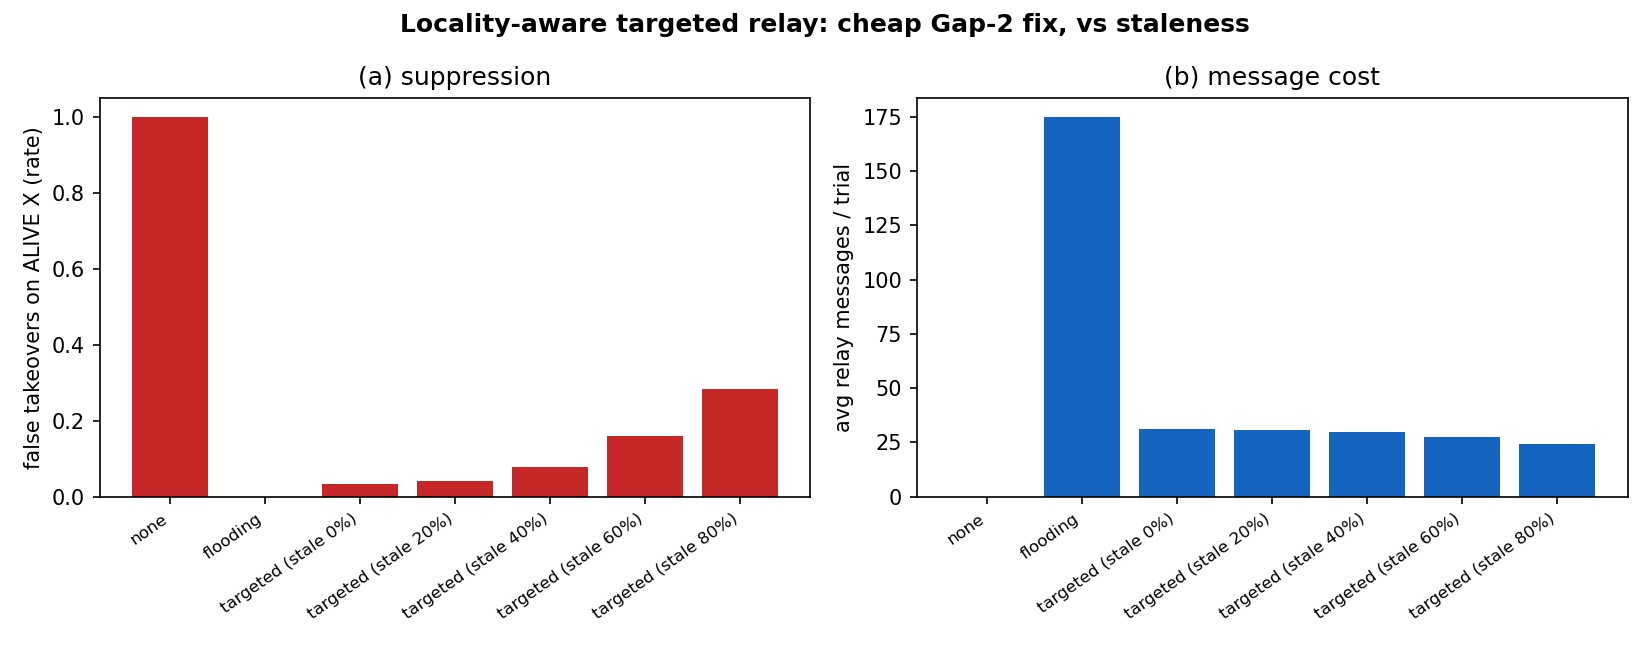
\includegraphics[width=\columnwidth]{fig_relay.png}
\caption{Per-robot heterogeneity (an alive robot occluded from its monitor).
(a)~suppression of false takeovers and (b)~message cost. Locality-targeted
indirect probing matches a full flood's suppression at $\sim$$1/6$ the cost and
degrades gracefully as the position model becomes stale.}
\label{fig:relay}
\end{figure}

\subsection{Embodied demonstration in a 3D surface-vessel simulator}
\label{sec:holoocean}
The results above are Monte Carlo studies over an abstract channel and point-mass
robots. To check that the mechanism behaves as designed once robots have physical
dynamics and travel real distances, we embodied it in HoloOcean (Unreal-based) on
a team of five SurfaceVessels performing a coverage-and-retrieval mission: every
point of interest (POI) must be searched, and a subset contain a retrievable item.
A monitor vessel runs both detectors live---$\varphi$-accrual as a logged shadow
and our belief $\beta=\rho\eta$ as the controller---over the same Gilbert--Elliott
heartbeat channel, with the re-allocation backend (Alg.~\ref{alg:backend}) and the
locality-targeted relay (Alg.~\ref{alg:relay}) closing the loop. We script three
ground-truth events so the comparison is auditable: a team-wide burst outage
(correlated silence), a genuine vessel failure under a healthy channel, and a
single-link partition of an alive vessel (the heterogeneity case of
Section~\ref{sec:relay}). The detection code is shared verbatim with the
Monte Carlo harness.

This is a qualitative single-run demonstration, not an additional statistical
claim. In a representative run (16 POIs, 6 items, all searched), our detector
incurred zero false takeovers while $\varphi$-accrual would have wrongly seized
four alive vessels during the correlated outage; the genuine failure was recovered
by re-allocation, and the partitioned-but-alive vessel triggered the relay, which
heard it through a neighbor and cancelled the takeover. The embodied behavior thus
reproduces, qualitatively, the false-takeover suppression, correct recovery, and
Gap-2 remedy characterized statistically above.

\section{Conclusion}
We presented a channel-aware failure recovery method for decentralized MRTA that
interprets silence through its correlation across the team. The standard per-node
detector suffers a false-takeover storm that \emph{grows linearly} with team
size---reaching $\sim$$25\times$ at $32$ robots---and a false-alarm floor it
provably cannot cross under correlated loss; our detector eliminates the storm,
is Pareto-dominant on detection latency at every matched operating point in the
practical regime, and carries that advantage downstream into wasted mission
energy. Its sequential form (Section~\ref{sec:seq}) further unifies the
per-node and channel-aware detectors as limiting cases and extends the safe
operating regime to a zero-miss, conflict-averse point whose advantage grows with
team size. The contribution is the principle and its empirical characterization
across $10^{2}$--$10^{3}$ trials, not a tuned formula.

\subsection{Future work}
\label{sec:future}
Several directions extend the sequential test of Section~\ref{sec:seq} beyond the
regime characterized here. The first is a full characterization across
\emph{graded} and \emph{flickering} channels---transient partitions and rapid
state changes in which channel health is no longer bimodal---together with online
channel-state estimation from timestamped broadcasts and reported confidence
intervals. A second is to carry the channel-coupled view from the failure
\emph{detection} decision to the upstream \emph{allocation} decision, where a
different signal than team-wide channel health may be required. Beyond these,
hardware validation on a physical team and cascading-failure scenarios, in which
a successor may itself fail, are natural next steps.

\bibliographystyle{IEEEtran}
\bibliography{references}

\end{document}
